%% Standalone figure for the Statistical Mechanics exercises (Quiz 1).
%% Build: pdflatex quiz1_sol_ternary.tex  (or run build.sh in this folder)
\documentclass[11pt,tikz,border=2pt]{standalone}
\usepackage{amsmath,amssymb}
\usetikzlibrary{arrows.meta, positioning}
\begin{document}
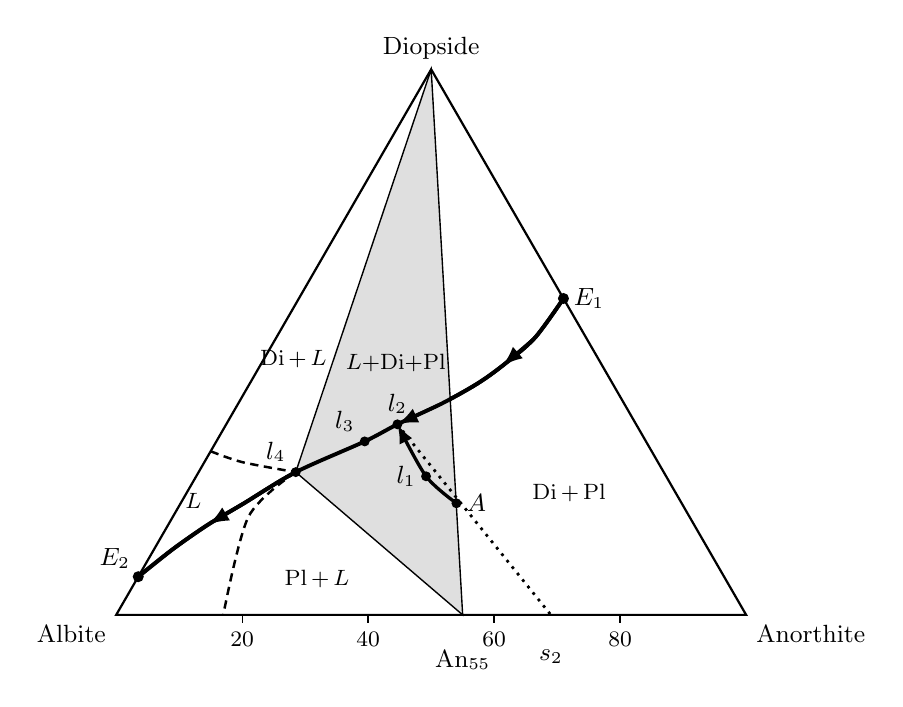
\begin{tikzpicture}[font=\small, >=Latex, line width=0.8pt]
    % corners and frame
    \coordinate (Ab) at (0,0);
    \coordinate (An) at (8,0);
    \coordinate (Di) at (4,6.928);
    \draw (Ab) -- (An) -- (Di) -- cycle;
    \node[below left] at (Ab) {Albite};
    \node[below right] at (An) {Anorthite};
    \node[above] at (Di) {Diopside};
    \foreach \p in {20,40,60,80}
        \draw[line width=0.5pt] (0.08*\p,0) -- (0.08*\p,-0.1) node[below, font=\footnotesize] {\p};
    % cotectic (boundary between the diopside and plagioclase fields)
    \draw[line width=1.4pt] plot[smooth] coordinates {(0.280,0.485) (0.728,0.841) (1.171,1.149) (1.614,1.412) (2.280,1.813) (3.156,2.203) (3.571,2.420) (4.135,2.684) (4.579,2.932) (4.903,3.162) (5.314,3.515) (5.680,4.018)};
    % three-phase tie triangle Di - l4 - plagioclase An55 (L + Di + Pl)
    \fill[gray!25] (Di) -- (2.280,1.813) -- (4.400,0.000) -- cycle;
    \draw[line width=0.5pt] (Di) -- (2.280,1.813) -- (4.400,0.000) -- cycle;
    \draw[line width=1.4pt] plot[smooth] coordinates {(0.280,0.485) (0.728,0.841) (1.171,1.149) (1.614,1.412) (2.280,1.813) (3.156,2.203) (3.571,2.420) (4.135,2.684) (4.579,2.932) (4.903,3.162) (5.314,3.515) (5.680,4.018)};
    % temperature falls along the cotectic from E1 to E2
    \draw[-{Latex[length=2.6mm]}, line width=1.2pt] (5.314,3.515) -- (4.903,3.162);
    \draw[-{Latex[length=2.6mm]}, line width=1.2pt] (4.135,2.684) -- (3.571,2.420);
    \draw[-{Latex[length=2.6mm]}, line width=1.2pt] (1.614,1.412) -- (1.171,1.149);
    \fill (5.680,4.018) circle (2pt) node[right] {$E_1$};
    \fill (0.280,0.485) circle (2pt) node[above left=-1pt] {$E_2$};
    % isotherm through l4: diopside-field branch and plagioclase-field branch
    \draw[line width=0.9pt, densely dashed] plot[smooth] coordinates {(1.200,2.078) (1.600,1.940) (2.280,1.813)};
    \draw[line width=0.9pt, densely dashed] plot[smooth] coordinates {(2.280,1.813) (1.680,1.247) (1.360,0.000)};
    % path of the liquid: A -> l1 -> l2 (plagioclase only), then l2 -> l4 on the cotectic
    \draw[line width=1.2pt, -{Latex[length=2.4mm]}] plot[smooth] coordinates {(4.321,1.417) (3.935,1.760) (3.571,2.420)};
    \draw[dotted, line width=1pt] (3.571,2.420) -- (5.520,0.000);
    \foreach \P/\n/\pos in {(4.321,1.417)/A/right, (3.935,1.760)/l_1/left, (3.571,2.420)/l_2/above, (3.156,2.203)/l_3/above left, (2.280,1.813)/l_4/above left}
        { \fill \P circle (1.8pt); \node[\pos] at \P {$\n$}; }
    \node[below=9pt] at (5.520,0.000) {$s_2$};
    \node[below=9pt] at (4.400,0.000) {An$_{55}$};
    % field labels
    \begin{scope}[font=\footnotesize]
        \node at (3.55,3.2) {$L$+Di+Pl};
        \node at (2.25,3.25) {Di$\,+\,L$};
        \node at (2.55,0.45) {Pl$\,+\,L$};
        \node at (5.75,1.55) {Di$\,+\,$Pl};
        \node at (0.98,1.45) {$L$};
    \end{scope}
\end{tikzpicture}
\end{document}
